\lab{Image Segmentation}{Image Segmentation}

\objective{Graph theory has a variety of applications.
A graph (or network) can be represented in many ways on a computer.
In this lab, we study a common matrix representation for graphs and show how certain properties of the matrix representation correspond to inherent properties of the original graph.
% In this lab, we learn to represent a graph as a matrix and to calculate properties of the graph using the matrix representation.
We also introduce tools for working with images in Python, and conclude with an application of using graphs and linear algebra to segment images.
}

\section*{Graphs as Matrices} % ===============================================

A \emph{graph} is a mathematical structure that represents relationships between objects.
Graphs are defined by $G = (V,E)$, where $V$ is a set of \emph{vertices} (or \emph{nodes}) and $E$ is a set of \emph{edges}, each of which connects one node to another.
A graph can be classified in several ways.
\begin{itemize}
    \item The edges of an \emph{undirected} graph are bidirectional: if an edge goes from node $A$ to node $B$, then that same edge also goes from $B$ to $A$.
    For example, the graphs $G_1$ and $G_2$ in Figure \ref{fig:imgseg-example-graphs} are both undirected.
    In a \emph{directed graph}, edges only go one way, usually indicated by an arrow pointing from one node to another.
    In this lab, we focus on undirected graphs.

    \item The edges of a \emph{weighted} graph have a weight assigned to them, such as $G_2$.
    A weighted graph could represent a collection of cities with roads connecting them: each vertex would represent a city, and the edges would represent roads between the cities.
    The length of each road could be the weight of the corresponding edge.
    An \emph{unweighted} graph like $G_1$ does not have weights assigned to its edges, but any unweighted graph can be thought of as a weighted graph by assigning a weight of $1$ to every edge.

    % \item A graph is \emph{simple} if no edge connects a node to itself.
    % The graph in Figure [TODO] is simple, but the graph in Figure [TODO] is not.
\end{itemize}

\begin{figure}[H] % Two graphs.
\captionsetup[subfigure]{justification=centering}
\centering
\begin{subfigure}{.45\textwidth}
    \centering
    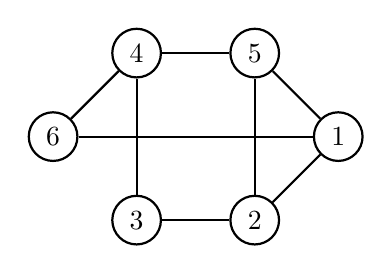
\begin{tikzpicture}[auto,node distance=1.5cm,
     thick,main node/.style={circle,draw}]

      \node[main node] (5) [] {6};
      \node[main node] (2) [below right of=5] {3};
      \node[main node] (3) [above right of=5] {4};
      \node[main node] (4) [right of=3] {5};
      \node[main node] (1) [right of=2] {2};
      \node[main node] (0) [below right of=4] {1};

      \foreach \s/\t in {5/3, 3/4, 4/0, 0/1, 1/2, 2/3, 1/4, 5/0} {
       \path[draw] (\s) edge (\t);}
    \end{tikzpicture}
    \caption{$G_1$, an unweighted undirected graph.}
    \label{fig:graphexample-unweighted}
\end{subfigure}
\quad
\begin{subfigure}{.45\textwidth}
    \centering
    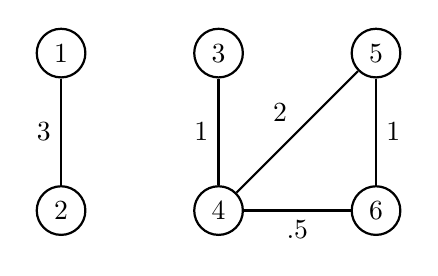
\begin{tikzpicture}[auto,node distance=2cm,
    thick,main node/.style={circle,draw}]

    \node[main node] (0) [] {1};
    \node[main node] (1) [below of=0] {2};
    \node[main node] (2) [right of=0] {3};
    \node[main node] (3) [below of=2] {4};
    \node[main node] (4) [right of=2] {5};
    \node[main node] (5) [right of=3] {6};

    \path[draw] (0) edge node [left] {3} (1);
    \path[draw] (2) edge node [left] {1} (3);
    \path[draw] (4) edge node{1} (5);
    \path[draw] (3) edge node{2} (4);
    \path[draw] (3) edge node [below]{.5} (5);
    \end{tikzpicture}
    \caption{$G_2$, a weighted undirected graph.}
    \label{fig:graphexample-weighted}
\end{subfigure}
% \qquad
% \begin{subfigure}{.28\textwidth}
%     \begin{tikzpicture}[->,>=stealth',shorten >=1pt,auto,node distance=1.5cm,
%     thick,main node/.style={circle,draw}]
%
%      \node[main node] (A) [] {A};
%      \node[main node] (B) [below of=A] {B};
%      \node[main node] (C) [right of=A] {C};
%      \node[main node] (D) [below of=C] {D};
%      \node[main node] (E) [right of=C] {E};
%      \node[main node] (F) [right of=D] {F};
%
%      \foreach \s/\t in {A/C, B/A, B/D, C/E, C/F, D/C} {
%       \path[draw] (\s) edge (\t);}
%     \end{tikzpicture}
%     \caption{A directed graph.}
% \end{subfigure}
\caption{}
\label{fig:imgseg-example-graphs}
\end{figure}

\subsection*{Adjacency, Degree, and Laplacian Matrices} % ---------------------

For computation and analysis, graphs are commonly represented by a few special matrices.
For these definitions, let $G$ be a graph with $N$ nodes and let $w_{ij}$ be the weight of the edge connecting node $i$ to node $j$ (if such an edge exists).
%
\begin{enumerate}
\item The \emph{adjacency matrix} of $G$ is the $N\times N$ matrix $A$ with entries
\[
a_{ij} =
\begin{cases}
w_{ij} & \text{if an edge connects node i and node j} \\
0 & \text{otherwise.}
\end{cases}
\]
% If the graph is not simple, there are differing conventions for how to define the diagonal of the adjacency matrix.
The adjacency matrices $A_1$ of $G_1$ and $A_2$ of $G_2$ are
\begin{align*}
A_1 = \left[\begin{array}{cccccc}
0 & 1 & 0 & 0 & 1 & 1\\
1 & 0 & 1 & 0 & 1 & 0\\
0 & 1 & 0 & 1 & 0 & 0\\
0 & 0 & 1 & 0 & 1 & 1\\
1 & 1 & 0 & 1 & 0 & 0\\
1 & 0 & 0 & 1 & 0 & 0
\end{array}\right],
\qquad A_2 =
\left[\begin{array}{cccccc}
0 & 3 & 0 & 0 & 0 & 0\\
3 & 0 & 0 & 0 & 0 & 0\\
0 & 0 & 0 & 1 & 0 & 0\\
0 & 0 & 1 & 0 & 2 & .5\\
0 & 0 & 0 & 2 & 0 & 1\\
0 & 0 & 0 & .5 & 1 & 0
\end{array}\right].
\end{align*}
Notice that these adjacency matrices are symmetric.
This is always the case for undirected graphs since the edges are bidirectional.

\begin{comment} % Paths of a certain length via matrix powers. Not relevant. ==
Raising the adjacency matrix to a power yields some very interesting information.
We can discover the number of paths of length $n$ between two nodes by raising a graph's adjacency matrix to the $n$th power.
For example, by squaring $A$, we can find the number of paths of length two between every pair of nodes.
\begin{lstlisting}
>>> A = np.array([[0,1,0,0,1,0],[1,0,1,0,1,0],
                  [0,1,0,1,0,0],[0,0,1,0,1,1],
                  [1,1,0,1,0,0],[0,0,0,1,0,0]])

>>> np.linalg.matrix_power(A,2)
array([[2, 1, 1, 1, 1, 0],
       [1, 3, 0, 2, 1, 0],
       [1, 0, 2, 0, 2, 1],
       [1, 2, 0, 3, 0, 0],
       [1, 1, 2, 0, 3, 1],
       [0, 0, 1, 0, 1, 1]])
\end{lstlisting}
We can see that no paths of length two exist between node 0 and node 5 because $A^2_{0,5} = 0$.
By calculating $A^6$ we can find the number of paths of length six from node 3 to itself.
\begin{lstlisting}
>>> np.linalg.matrix_power(A, 6)
array([[45, 54, 38, 45, 54, 16],
       [54, 86, 29, 77, 51, 11],
       [38, 29, 55, 15, 70, 27],
       [45, 77, 15, 75, 31,  4],
       [54, 51, 70, 31, 93, 34],
       [16, 11, 27,  4, 34, 14]])
\end{lstlisting}
Therefore there are 75 unique paths of length six from node 3 to itself.
Imagine trying to count all of those paths by hand!
It would be very easy to count incorrectly.
This method makes it very simple to count paths without mistakes.

Adjacency matrices can also be composed of \li{True} and \li{False} values.
In this case, the $n$th power of such a matrix (using boolean arithmetic)
is again a matrix of
boolean values which simply indicate whether there exists a path of length $n$ between the given pair of nodes, rather than indicating the number of such
paths.

\begin{problem}
Let the following matrix represent a directed graph
\[
\begin{array}{ccccccc}
0 & 0 & 1 & 0 & 1 & 0 & 1 \\
1 & 0 & 0 & 0 & 0 & 1 & 0 \\
0 & 0 & 0 & 0 & 0 & 1 & 0 \\
1 & 0 & 0 & 0 & 1 & 0 & 0 \\
0 & 0 & 0 & 1 & 0 & 0 & 0 \\
0 & 0 & 1 & 0 & 0 & 0 & 1 \\
0 & 1 & 0 & 0 & 0 & 0 & 0
\end{array}\right]
\]
Between which pair of nodes does there exist the greatest number of paths
of length five?
From which node to which node is there no path of length seven?
\end{problem}
\end{comment} % ===============================================================

\item The \emph{degree matrix} of $G$ is the $N \times N$ diagonal matrix $D$ whose $i$th diagonal entry is
\begin{equation}
d_{ii} = \sum_{j=1}^N w_{ij}.
\label{eq:degree-matrix-formula}
\end{equation}
%For a directed graph, each node has an \emph{out-degree} (the number of edges directed away from a node) and an \emph{in-degree} (the number edges directed toward a node).
The degree matrices $D_1$ of $G_1$ and $D_2$ of $G_2$ are
\begin{align*}
D_1 = \left[\begin{array}{cccccc}
3 & 0 & 0 & 0 & 0 & 0\\
0 & 3 & 0 & 0 & 0 & 0\\
0 & 0 & 2 & 0 & 0 & 0\\
0 & 0 & 0 & 3 & 0 & 0\\
0 & 0 & 0 & 0 & 3 & 0\\
0 & 0 & 0 & 0 & 0 & 2
\end{array}\right],
\qquad D_2 =
\left[\begin{array}{cccccc}
3 & 0 & 0 & 0 & 0 & 0\\
0 & 3 & 0 & 0 & 0 & 0\\
0 & 0 & 1 & 0 & 0 & 0\\
0 & 0 & 0 & 3.5 & 0 & 0\\
0 & 0 & 0 & 0 & 3 & 0\\
0 & 0 & 0 & 0 & 0 & 1.5
\end{array}\right].
\end{align*}
The $i$th diagonal entry of $D$ is called the \emph{degree} of node $i$, the sum of the weights of the edges leaving node $i$.

\item The \emph{Laplacian matrix} of $G$ is the $N\times N$ matrix $L$ defined as
\begin{equation}
L = D - A,
\label{eq:laplacian-matrix-formula}
\end{equation}
where $D$ is the degree matrix of $G$ and $A$ is the adjacency matrix of $G$.
For $G_1$ and $G_2$, the Laplacian matrices $L_1$ and $L_2$ are
\begin{align*}
L_1 =\left[\begin{array}{rrrrrr}
3 & -1 & 0 & 0 & -1 & -1\\
-1 & 3 & -1 & 0 & -1 & 0\\
0 & -1 & 2 & -1 & 0 & 0\\
0 & 0 & -1 & 3 & -1 & -1\\
-1 & -1 & 0 & -1 & 3& 0\\
-1 & 0 & 0 & -1 & 0 & 2
\end{array}\right],
\qquad L_2 =
 \left[\begin{array}{rrrrrr}
3 & -3 & 0 & 0 & 0 & 0\\
-3 & 3 & 0 & 0 & 0 & 0\\
0 & 0 & 1 & -1 & 0 & 0\\
0 & 0 & -1 & 3.5 & -2 & -.5\\
0 & 0 & 0 & -2 & 3 & -1\\
0 & 0 & 0 &- .5 & -1 & 1.5
\end{array}\right].
\end{align*}
\end{enumerate}

\begin{problem}
Write a function that accepts the adjacency matrix $A$ of a graph $G$.
Use (\ref{eq:degree-matrix-formula}) and (\ref{eq:laplacian-matrix-formula}) to compute the Laplacian matrix $L$ of $G$.
\\(Hint: The diagonal entries of $D$ can be computed in one line by summing $A$ over an axis.)

Test your function on the graphs $G_1$ and $G_2$ from Figure \ref{fig:imgseg-example-graphs} and validate your results with \li{scipy.sparse.csgraph.laplacian()}.
\label{prob:imgseg-laplacian}
\end{problem}

\subsection*{Connectivity} % --------------------------------------------------

A \emph{connected graph} is a graph where every vertex is connected to every other vertex by at least one path.
For example, $G_1$ is connected, whereas $G_2$ is not because there is no path from node $1$ (or node $2$) to node $3$ (or nodes $4$, $5$, or $6$).
The na\"ive brute-force algorithm for determining if a graph is connected is to check that there is a path from each edge to every other edge.
While this may work for very small graphs, most interesting graphs have thousands of vertices, and for such graphs this approach is prohibitively expensive.
Luckily, an interesting result from algebraic graph theory relates the connectivity of a graph to its Laplacian matrix.

If $L$ is the Laplacian matrix of a graph, then the definition of $D$ and the construction $L = D - A$ guarantees that the rows (and columns) of $L$ must each sum to $0$.
Therefore $L$ cannot have full rank, so $\lambda = 0$ must be an eigenvalue of $L$.
Furthermore, if $L$ represents a graph that is \textbf{not} connected, more than one of the eigenvalues of $L$ must be zero.
To see this, let $J \subset \{1,2,\ldots,N\}$ such that the vertices $\{v_j\}_{j \in J}$ form a connected component of the graph, meaning that there is a path between each pair of vertices in the set.
Next, let $\x$ be the vector with entries
 \[
x_k = \begin{cases}
1, & k \in J    \\
0, & k \not\in J.
\end{cases}
  \]
Then $\x$ is an eigenvector of $L$ corresponding to the eigenvalue $\lambda = 0$.
% In other words, for each connected component, $0$ appears at least once as an eigenvalue.

For example, the example graph $G_2$ has two connected components.
\begin{enumerate}
\item $J_1 = \{1,2\}$ so that $\x_1 = [1, 1, 0, 0, 0, 0]\trp$.
Then
\[
L_2\x_1 =
\left[\begin{array}{rrrrrr}
3 & -3 & 0 & 0 & 0 & 0\\
-3 & 3 & 0 & 0 & 0 & 0\\
0 & 0 & 1 & -1 & 0 & 0\\
0 & 0 & -1 & 3.5 & -2 & -.5\\
0 & 0 & 0 & -2 & 3 & -1\\
0 & 0 & 0 &- .5 & -1 & 1.5
\end{array}\right]
\left[\begin{array}{c}
1 \\ 1 \\ 0 \\ 0 \\ 0 \\ 0
\end{array}\right]
=
\left[\begin{array}{c}
0 \\ 0 \\ 0 \\ 0 \\ 0 \\ 0
\end{array}\right]
= \0.
\]

\item $J_2 = \{3,4,5,6\}$ and hence $\x_2 = [0, 0, 1, 1, 1, 1]\trp$.
Then
\[
L_2\x_2 =
\left[\begin{array}{rrrrrr}
3 & -3 & 0 & 0 & 0 & 0\\
-3 & 3 & 0 & 0 & 0 & 0\\
0 & 0 & 1 & -1 & 0 & 0\\
0 & 0 & -1 & 3.5 & -2 & -.5\\
0 & 0 & 0 & -2 & 3 & -1\\
0 & 0 & 0 &- .5 & -1 & 1.5
\end{array}\right]
\left[\begin{array}{c}
0 \\ 0 \\ 1 \\ 1 \\ 1 \\ 1
\end{array}\right]
=
\left[\begin{array}{c}
0 \\ 0 \\ 0 \\ 0 \\ 0 \\ 0
\end{array}\right]
= \0.
\]
\end{enumerate}

In fact, it can be shown that the number of zero eigenvalues of the Laplacian exactly equals the number of connected components.
This makes calculating how many connected components are in a graph only as hard as calculating the eigenvalues of its Laplacian.

A Laplacian matrix $L$ is always a positive semi-definite matrix when all weights in the graph are positive, meaning that its eigenvalues are each nonnegative.
The second smallest eigenvalue of $L$ is called the \emph{algebraic connectivity} of the graph.
It is clearly $0$ for non-connected graphs, but for a connected graph, the algebraic connectivity provides useful information about its sparsity or ``connectedness.''
A higher algebraic connectivity indicates that the graph is more strongly connected.

\begin{problem}
Write a function that accepts the adjacency matrix $A$ of a graph $G$ and a small tolerance value \li{tol}.
Compute the number of connected components in $G$ and its algebraic connectivity.
Consider all eigenvalues that are less than the given \li{tol} to be zero.

Use \li{scipy.linalg.eig()} or \li{scipy.linalg.eigvals()} to compute the eigenvalues of the Laplacian matrix.
These functions return complex eigenvalues (with negligible imaginary parts); use \li{np.real()} to extract the real parts.
\end{problem}

\begin{comment} % Likelihood of connectedness.
\begin{problem}
% Used to be part of the previous problem.
% Rmoved because these is no great way to evaluate it.
The folowing function creates a random symmetric matrix of Boolean values with sparsity determined by the input \li{c}.
\begin{lstlisting}
def sparse_generator(n, c):
    """Return a symmetric nxn matrix with sparsity determined by c."""
    A = np.random.rand(n**2).reshape((n, n))
    A = ( A > c**(.5) )
    return A.T @ A
\end{lstlisting}

Test your function from the previous problem on matrices created by \li{sparse_generator()} with inputs $n = 10, 100$ and $c = .25, .5, .95$.
What do you notice about the likelihood that a random graph is connected?
\end{problem}
\end{comment}

\section*{Images as Matrices} % ===============================================

Computer images are stored as arrays of integers that indicate pixel values.
Most $m\times n$ grayscale (black and white) images are stored in Python as a $m\times n$ NumPy arrays, while most $m\times n$ color images are stored as $3$-dimensional $m\times n \times 3$ arrays.
Color image arrays can be thought of as a stack of three $m\times n$ arrays, one each for red, green, and blue values.
% \footnote{See \url{http://scikit-image.org/docs/dev/user_guide/numpy_images.html\#coordinate-conventions} for other conventions.}
The datatype for an image array is \li{np.uint8}, unsigned 8-bit integers that range from $0$ to $255$.
A $0$ indicates a black pixel while a $255$ indicates a white pixel.

Use \li{imageio.imread()} to read an image from a file and \li{imageio.imwrite()} to save an image.
Matplotlib's \li{plt.imshow()} displays an image array, but it displays arrays of floats between $0$ and $1$ more cleanly than arrays of 8-bit integers.
Therefore it is customary to scale the array by dividing each entry by $255$ before processing or showing the image.
In this case, a $0$ still indicates a black pixel, but now a $1$ indicates pure white.

\begin{lstlisting}
>>> from imageio import imread
>>> from matplotlib import pyplot as plt

>>> image = imread("dream.png")     # Read a (very) small image.
>>> print(image.shape)              # Since the array is 3-dimensional,
(48, 48, 3)                         # this is a color image.

# The image is read in as integers from 0 to 255.
>>> print(image.<<min>>(), image.<<max>>(), image.dtype)
0 254 uint8

# Scale the image to floats between 0 and 1 for Matplotlib.
>>> scaled = image / 255.
>>> print(scaled.<<min>>(), scaled.<<max>>(), scaled.dtype)
0.0 0.996078431373 float64

# Display the scaled image.
>>> plt.imshow(scaled)
>>> plt.axis("off")
\end{lstlisting}

A color image can be converted to grayscale by averaging the RGB values of each pixel, resulting in a 2-D array called the \emph{brightness} of the image.
To properly display a grayscale image, specify the keyword argument \li{cmap="gray"} in \li{plt.imshow()}.

\begin{lstlisting}
# Average the RGB values of a colored image to obtain a grayscale image.
>>> brightness = scaled.mean(axis=2)        # Average over the last axis.
>>> print(brightness.shape)                 # Note that the array is now 2-D.
(48, 48)

# Display the image in gray.
>>> plt.imshow(brightness, cmap="gray")
>>> plt.axis("off")
\end{lstlisting}

Finally, it is often important in applications to flatten an image matrix into a large 1-D array.
Use \li{np.ravel()} to convert a $m\times n$ array into a 1-D array with $mn$ entries.

\begin{lstlisting}
>>> import numpy as np
>>> A = np.random.randint(0, 10, (3,4))
>>> print(A)
[[4 4 7 7]
 [8 1 2 0]
 [7 0 0 9]]

# Unravel the 2-D array (by rows) into a 1-D array.
>>> np.ravel(A)
array([4, 4, 7, 7, 8, 1, 2, 0, 7, 0, 0, 9])

# Unravel a grayscale image into a 1-D array and check its size.
>>> M,N = brightness.shape
>>> flat_brightness = np.ravel(brightness)
>>> M*N == flat_brightness.size
<<True>>
>>> print(flat_brightness.shape)
(2304,)
\end{lstlisting}

\begin{problem} % Read and display an image.
Define a class called \li{ImageSegmenter}.
\begin{enumerate}
    \item Write the constructor so that it accepts the name of an image file.
    Read the image, scale it so that it contains floats between $0$ and $1$, then store it as an attribute.
    If the image is in color, compute its brightness matrix by averaging the RGB values at each pixel (if it is a grayscale image, the image array itself is the brightness matrix).
    Flatten the brightness matrix into a 1-D array and store it as an attribute.

    \item Write a method called \li{show_original()} that displays the original image.
    If the original image is grayscale, remember to use \li{cmap="gray"} as part of \li{plt.imshow()}.
\end{enumerate}
\end{problem}

\begin{warn} % Do not use plt.imread() because it is inconsistent.
Matplotlib's \li{plt.imread()} also reads image files.
However, this function automatically scales PNG image entries to floats between $0$ and $1$, but it still reads non-PNG image entries as 8-bit integers.
To avoid this inconsistent behavior, always use \li{imageio.imread()} to read images and divide by $255$ when scaling is desired.
\end{warn}

\section*{Graph-based Image Segmentation} % ===================================

\emph{Image segmentation} is the process of finding natural boundaries in an image and partitioning the image along those boundaries (see Figure \ref{fig:imgseg-segmentation-example}).
Though humans can easily pick out portions of an image that ``belong together,'' it takes quite a bit of work to teach a computer to recognize boundaries and sections in an image.
However, segmenting an image often makes it easier to analyze, so image segmentation is ongoing area of research in computer vision and image processing.

\begin{figure}[H] % Segmentation example.
    \centering
    \begin{subfigure}{.32\textwidth}
        \includegraphics[width=\textwidth]{figures/dream.pdf}
    \end{subfigure}
    %
    \begin{subfigure}{.32\textwidth}
        \includegraphics[width=\textwidth]{figures/dream_pos.pdf}
    \end{subfigure}
    %
    \begin{subfigure}{.32\textwidth}
        \includegraphics[width=\textwidth]{figures/dream_neg.pdf}
    \end{subfigure}
\caption{The image \texttt{dream.png} and its segments.}
\label{fig:imgseg-segmentation-example}
\end{figure}

There are many ways to approach image segmentation.
The following algorithm, developed by Jianbo Shi and Jitendra Malik in 2000 \cite{Shi2000}, converts the image to a graph and ``cuts'' it into two connected components.

\subsection*{Constructing the Image Graph} % ----------------------------------

Let $G$ be a graph whose vertices are the $mn$ pixels of an $m\times n$ image (either grayscale or color).
% That is, vertex $i$ in $G$ represents the pixel at index $i$ when the image is flattened to a vector with $mn$ entries.
Each vertex $i$ has a brightness $B(i)$, the grayscale or average RGB value of the pixel, as well as a coordinate location $X(i)$, the indices of the pixel in the original image array.

Define $w_{ij}$, the weight of the edge between pixels $i$ and $j$, by
\begin{equation}
\label{eq:imgseg-edge-weight}
w_{ij} = \begin{cases}
\exp\left(-\frac{|B(i) - B(j)|}{\sigma_B^2}-\frac{\|X(i) - X(j)\|}{\sigma_X^2}\right) & \text{if}\ \|X(i) - X(j)\| < r \\ 0 & \text{otherwise,}
\end{cases}
\end{equation}
where $r$, $\sigma_B^2$ and $\sigma_X^2$ are constants for tuning the algorithm.
In this context, $\|\cdot\|$ is the standard \emph{euclidean norm}, meaning that $\|X(i) - X(j)\|$ is the physical distance between vertices $i$ and $j$, measured in pixels.

With this definition for $w_{ij}$, pixels that are farther apart than the radius $r$ are not connected at all in $G$.
Pixels within $r$ of each other are more strongly connected if they are similar in brightness and close together (the value in the exponential is negative but close to zero).
On the other hand, highly contrasting pixels where $|B(i) - B(j)|$ is large have weaker connections (the value in the exponential is highly negative).

\begin{figure}[H] % The adjacency matrix. DO NOT DELETE. EVER.
\begin{tikzpicture}[dot/.style={circle,fill=black,minimum
    size=4pt,inner sep=0pt,outer sep=-1pt}, >=stealth]
%scale=.85, transform shape,

%image
\draw[step=.75,thick](2.999,0)grid(6,3);
%numbers 1-16
\foreach \x in {0,1,2,3}
    \foreach \y in {4}
        \node[draw=none, anchor=south west]at(\x*.75+3.25, \y-1.4){\x};
\foreach \x [evaluate=\x as \r using int(\x+4)]in {0,1,2,3}
    \foreach \y in {3}
        \node[draw=none, anchor=south west]at(\x*.75+3.25, \y-1.2){\r};
\foreach \x [evaluate=\x as \r using int(\x+8)] in {0,1,2,3}
    \foreach \y in {2}
        \node[draw=none, anchor=south west]at(\x*.75+3.25, \y-.95){\r};
\foreach \x [evaluate=\x as \r using int(\x+12)] in {0,1,2,3}
    \foreach \y in {1}
        \node[draw=none, anchor=south west]at(\x*.75+3.25, \y-.7){\r};

\node[draw=none](image)at(4.5, -.5){\emph{image}};
\node[draw=none](flattened)at(7.25,-3){\emph{flattened image}};
\node[draw=none](adjacency)at(12,-3){\emph{adjacency matrix} $A$};

%dots within grid
\foreach \x in {1,2,3,4}
    \foreach \y in {1,2,3,4}
        \node[draw, dot]at(\x*.75+2.6,\y*.75-.4){};

%color fill
\foreach \x/\y in {2/3.75, 1.25/3, 2/3, 2.75/3, 2/2.25} {\node[draw, minimum
    size=.75cm, fill=green!30!black, fill opacity=.25]at(\x+2.118,\y-1.118){};}

%circle in image
\node[draw, circle, minimum size=2cm,thick](circle)at(4.13,1.86){};

%flattened image
\draw[step=.5, thick](6.999,-2.5)grid(7.5,5.5);
\foreach \x in {7}
    \foreach \y in {0,...,15}
        \node[draw=none]at(\x+.25,\y*-.5+5.25){\y};

\draw[->,thick](6.1, 1.5)--(6.9,1.5);

%adjancey matrix
\draw[step=.5](7.9999,-2.5)grid(16,5.5);
%\draw[step=2,thick](7.999,-2.5)grid(16,5.5);

%outside labels
\foreach \x in {0,4,8,12} {\node[draw=none]at(\x*.5+8.25,5.8){\x};}
\foreach \y in {0,4,8,12}{\node[draw=none]at(16.3,\y*-.5+5.3){\y};}

%shading of boxes
\foreach \x/\y in {8.5/5.5, 9/5.5, 8.5/5, 9/5, 9.5/5,9/4.5,9.5/4.5,10/4.5,
    9.5/4, 10/4, 10.5/5.5, 11/5,11.5/4.5, 12/4, 12.5/3.5,
    13.5/2.5, 14/2, 14.5/1.5, 15/1, 15.5/.5,16/0, 10.5/3.5, 11/3.5, 11/2.5,
    11.5/2.5,12/2.5, 11.5/2,12/2, 12.5/1.5, 13/1.5, 12.5/1, 13/1,
    13.5/1,13/.5,13.5/.5,14/.5, 13.5/0,14/0, 14.5/-.5,15/-.5,14.5/-1,
    15/-1,15.5/-1, 15/-1.5, 15.5/-1.5, 16/-1.5, 15.5/-2, 16/-2, 8.5/3.5,
    9.5/2.5,10/2,10.5/1.5,11/1,11.5/.5,12/0, 12.5/-.5, 13/-1, 13.5/-1.5, 14/-2}
    {\node[draw, minimum size=.5cm, fill=black, fill opacity=.25]
    at(\x-.25,\y-.25){};}

%green shaded boxes
\foreach \x/\y in {9/3,11/3, 11.5/3, 10.5/3, 13/3} {\node
    [draw, minimum size=.5cm, fill=shadecolor]
    at(\x-.25,\y-.25){};}

\node[draw=none]at(8.75,2.75){1};
\node[draw=none]at(10.25,2.75){4};
\node[draw=none]at(10.75,2.75){5};
\node[draw=none]at(11.25,2.75){6};
\node[draw=none]at(12.75,2.75){9};
\end{tikzpicture}

\caption{The grid on the left represents a $4\times4$ ($m \times n$) image with $16$ pixels.
On the right is the corresponding $16 \times 16$ ($mn \times mn$) adjacency matrix with all nonzero entries shaded.
For example, in row $5$, entries $1$, $4$, $5$, $6$, and $9$ are nonzero because those pixels are within radius $r=1.2$ of pixel $5$.}
\label{fig:imgseg-adjacency-tikz}
\end{figure}

Since there are $mn$ total pixels, the adjacency matrix $A$ of $G$ with entries $w_{ij}$ is $mn\times mn$.
With a relatively small radius $r$, $A$ is relatively sparse, and should therefore be constructed and stored as a sparse matrix.
The degree matrix $D$ is diagonal, so it can be stored as a regular 1-dimensional NumPy array.
The procedure for constructing these matrices can be summarized in just a few steps.
\begin{enumerate}
    \item Initialize $A$ as a sparse $mn\times mn$ matrix and $D$ as a vector with $mn$ entries.
    \item For each vertex $i$ ($i=0,1,\ldots,mn-1$),
    \begin{enumerate}
        \item Find the set of all vertices $J_i$ such that $\|X(i) - X(j)\| < r$ for each $j\in J_i$.
        For example, in Figure \ref{fig:imgseg-adjacency-tikz} $i=5$ and $J_i = \{1,4,5,6,9\}$.
        \label{step:imgseg-neighborhood}
        \item Calculate the weights $w_{ij}$ for each $j\in J_i$ according to (\ref{eq:imgseg-edge-weight}) and store them in $A$.
        \item Set the $i$th element of $D$ to be the sum of the weights, $d_i = \sum_{j\in J_i}w_{ij}$.
    \end{enumerate}
\end{enumerate}

The most difficult part to implement efficiently is step \ref{step:imgseg-neighborhood}, computing the neighborhood $J_i$ of the current pixel $i$.
However, the computation only requires knowing the current index $i$, the radius $r$, and the height and width $m$ and $n$ of the original image.
The following function takes advantage of this fact and returns (as NumPy arrays) both $J_i$ and the distances $\|X(i) - X(j)\|$ for each $j\in J_i$.

% get_neighbors() helper function.
\begin{lstlisting}
def get_neighbors(index, radius, height, width):
    """Calculate the flattened indices of the pixels that are within the given
    distance of a central pixel, and their distances from the central pixel.

    Parameters:
        index (int): The index of a central pixel in a flattened image array
            with original shape (radius, height).
        radius (float): Radius of the neighborhood around the central pixel.
        height (int): The height of the original image in pixels.
        width (int): The width of the original image in pixels.

    Returns:
        (1-D ndarray): the indices of the pixels that are within the specified
            radius of the central pixel, with respect to the flattened image.
        (1-D ndarray): the euclidean distances from the neighborhood pixels to
            the central pixel.
    """
    # Calculate the original 2-D coordinates of the central pixel.
    row, col = index // width, index % width

    # Get a grid of possible candidates that are close to the central pixel.
    r = int(radius)
    x = np.arange(max(col - r, 0), min(col + r + 1, width))
    y = np.arange(max(row - r, 0), min(row + r + 1, height))
    X, Y = np.meshgrid(x, y)

    # Determine which candidates are within the given radius of the pixel.
    R = np.sqrt(((X - col)**2 + (Y - row)**2))
    mask = R < radius
    return (X[mask] + Y[mask]*width).astype(np.<<int>>), R[mask]
\end{lstlisting}

To see how this works, consider Figure \ref{fig:imgseg-adjacency-tikz} where the original image is $4\times 4$ and the goal is to compute the neighborhood of the pixel $i = 5$.

\begin{lstlisting}
# Compute the neighbors and corresponding distances from the figure.
>>> neighbors_1, distances_1 = get_neighbors(5, 1.2, 4, 4)
>>> print(neighbors_1, distances_1, sep='\n')
[1 4 5 6 9]
[ 1.  1.  0.  1.  1.]

# Increasing the radius from 1.2 to 1.5 results in more neighbors.
>>> neighbors_2, distances_2 = get_neighbors(5, 1.5, 4, 4)
>>> print(neighbors_2, distances_2, sep='\n')
[ 0  1  2  4  5  6  8  9 10]
[ 1.41421356  1.          1.41421356  1.          0.          1.
  1.41421356  1.          1.41421356]
\end{lstlisting}

\begin{problem}
Write a method for the \li{ImageSegmenter} class that accepts floats $r$ defaulting to $5$, $\sigma_B^2$ defaulting to $.02$, and $\sigma_X^2$ defaulting to $3$.
Compute the adjacency matrix $A$ and the degree matrix $D$ according to the weights specified in (\ref{eq:imgseg-edge-weight}).

Initialize $A$ as a \li{scipy.sparse.lil_matrix}, which is optimized for incremental construction.
Fill in the nonzero elements of $A$ one row at a time.
Use \li{get_neighbors()} at each step to help compute the weights.
\\(Hint: Try to compute and store an entire row of weights at a time.
What does the command \li{A[5, np.array([1, 4, 5, 6, 9])] = weights} do?)

Finally, convert $A$ to a \li{scipy.sparse.csc_matrix}, which is faster for computations.
Then return $A$ and $D$.
\label{prob:imgseg-compute-adjacency}
\end{problem}

\subsection*{Segmenting the Graph} % ------------------------------------------

With an image represented as a graph $G$, the goal is to now split $G$ into two distinct connected components by removing edges from the existing graph.
This is called \emph{cutting} $G$, and the set of edges that are removed is called the \emph{cut}.
The cut with the least weight will best segment the image.

Let $D$ be the degree matrix and $L$ be the Laplacian matrix of $G$.
Shi and Malik \cite{Shi2000} proved that the eigenvector corresponding to the second smallest\footnote{Both $D$ and $L$ are symmetric matrices, so all eigenvalues of $D^{-1/2}LD^{-1/2}$ are real, and therefore ``the second smallest one'' is well-defined.} eigenvalue of $D^{-1/2}LD^{-1/2}$ can be used to minimize the cut: the indices of its positive entries are the indices of the pixels in the flattened image which belong to one segment, and the indices of its negative entries are the indices of the pixels which belong to the other segment.
In this context $D^{-1/2}$ refers to element-wise exponentiation, so the $(i,j)$th entry of $D^{-1/2}$ is $1/\sqrt{d_{ij}}$.

Because $A$ is $mn\times mn$, the desired eigenvector has $mn$ entries.
Reshaping the eigenvector to be $m \times n$ allows it to align with the original image.
Use the reshaped eigenvector to create a boolean mask that indexes one of the segments.
That is, construct a $m\times n$ array where the entries belonging to one segment are \li{True} and the other entries are \li{False}.

\begin{lstlisting}
>>> x = np.arange(-5,5).reshape((5,2)).T
>>> print(x)
[[-5 -3 -1  1  3]
 [-4 -2  0  2  4]]

# Construct a boolean mask of x describing which entries of x are positive.
>>> mask = x > 0
>>> print(mask)
<<[[False False False  True  True]
 [False False False  True  True]]>>

# Use the mask to zero out all of the nonpositive entries of x.
>>> x * mask
array([[0, 0, 0, 1, 3],
       [0, 0, 0, 2, 4]])
\end{lstlisting}

\begin{problem}
Write a method for the \li{ImageSegmenter} class that accepts an adjacency matrix $A$ as a \li{scipy.sparse.csc_matrix} and a degree matrix $D$ as a 1-D NumPy array.
Construct an $m\times n$ boolean mask describing the segments of the image.
\begin{enumerate}
    \item Compute the Laplacian $L$ with \li{scipy.sparse.csgraph.laplacian()} or by converting $D$ to a sparse diagonal matrix and computing $L = D - A$ (do not use your function from Problem \ref{prob:imgseg-laplacian} unless it works correctly and efficiently for sparse matrices).

    \item Construct $D^{-1/2}$ as a sparse diagonal matrix using $D$ and \li{scipy.sparse.diags()}, then compute $D^{-1/2}LD^{-1/2}$.
    Use \li{@} or the \li{dot()} method of the sparse matrix for the matrix multiplication, \textbf{not} \li{np.dot()}.

    \item Use \li{scipy.spase.linalg.eigsh()} to compute the eigenvector corresponding to the second-smallest eigenvalue of $D^{-1/2} L D^{-1/2}$.
    Set the keyword arguments \li{which="SM"} and \li{k=2} to compute only the two smallest eigenvalues and their eigenvectors.

    \item Reshape the eigenvector as a $m\times n$ matrix and use this matrix to construct the desired boolean mask.
    Return the mask.
\end{enumerate}
\label{prob:imgseg-compute-mask}
\end{problem}

Multiplying the boolean mask component-wise by the original image array produces the \emph{positive segment}, a copy of the original image where the entries that aren't in the segment are set to $0$.
Computing the \emph{negative segment} requires inverting the boolean mask, then multiplying the inverted mask with the original image array.
Finally, if the original image is a $m \times n \times 3$ color image, the mask must be stacked into a $m \times n \times 3$ array to facilitate entry-wise multiplication.

\begin{lstlisting}
>>> mask = np.arange(-5,5).reshape((5,2)).T > 0
>>> print(mask)
<<[[False False False  True  True]
 [False False False  True  True]]>>

# The mask can be negated with the tilde operator ~.
>>> print(~mask)
<<[[ True  True  True False False]
 [ True  True  True False False]]>>

# Stack a mask into a 3-D array with np.dstack().
>>> print(mask.shape, np.dstack((mask, mask, mask)).shape)
(2, 5) (2, 5, 3)
\end{lstlisting}

\begin{problem}
Write a method for the \li{ImageSegmenter} class that accepts floats $r$, $\sigma_B^2$, and $\sigma_X^2$, with the same defaults as in Problem \ref{prob:imgseg-compute-adjacency}.
Call your methods from Problems \ref{prob:imgseg-compute-adjacency} and \ref{prob:imgseg-compute-mask} to obtain the segmentation mask.
Plot the original image, the positive segment, and the negative segment side-by-side in subplots.
Your method should work for grayscale or color images.

Use \texttt{dream.png} as a test file and compare your results to Figure \ref{fig:imgseg-segmentation-example}.
\end{problem}

\begin{comment} % TODO

\newpage

\section*{Additional Material} % ==============================================

\subsection*{Products of Adjacency Matrices} % --------------------------------

\subsection*{Other Methods for Image Segmentation} % --------------------------

\end{comment}
